% Nature-style figure — pairwise relations grow quadratically with group size
% build: pdflatex fig-pairwise-growth.tex
\documentclass[border=2pt]{standalone}
\usepackage[T1]{fontenc}
\usepackage[scaled=1.0]{helvet}
\renewcommand{\familydefault}{\sfdefault}
\usepackage{amsmath}
\usepackage{sansmath}
\usepackage{anyfontsize}
\usepackage{xcolor}
\usepackage{tikz}
\usepackage{pgfplots}
\pgfplotsset{compat=1.18}
\usetikzlibrary{calc}

\definecolor{ink}{HTML}{1A1A1A}
\definecolor{acc}{HTML}{2F5D8C}
\definecolor{lgt}{HTML}{9FB8CD}
\definecolor{gry}{HTML}{8A8A8A}

\newcommand{\panellabel}[3]{\node[anchor=north west,font=\bfseries\fontsize{8}{9}\selectfont,
  text=ink] at (#1,#2) {#3};}

% \cgraph{center x}{center y}{N}{radius}
\newcommand{\cgraph}[4]{%
  \foreach \i in {1,...,#3}{%
    \foreach \j in {1,...,#3}{%
      \ifnum\i<\j
        \draw[lgt,line width=0.16pt]
          ({#1+#4*cos(90+(\i-1)*360/#3)},{#2+#4*sin(90+(\i-1)*360/#3)}) --
          ({#1+#4*cos(90+(\j-1)*360/#3)},{#2+#4*sin(90+(\j-1)*360/#3)});
      \fi}}%
  \foreach \i in {1,...,#3}{%
    \filldraw[fill=white,draw=acc,line width=0.28pt]
      ({#1+#4*cos(90+(\i-1)*360/#3)},{#2+#4*sin(90+(\i-1)*360/#3)}) circle (0.55);}%
}

\begin{document}
\sansmath\fontsize{7}{8.4}\selectfont
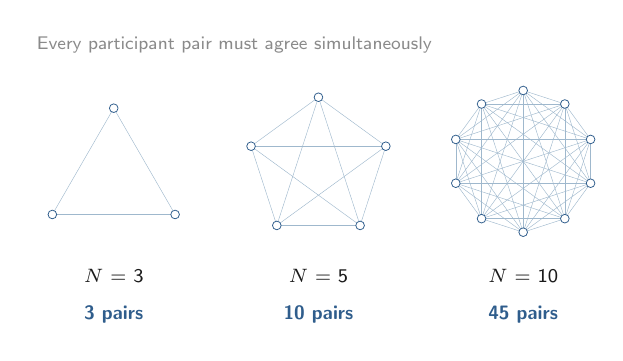
\begin{tikzpicture}[x=1mm,y=1mm,font=\fontsize{7}{8.4}\selectfont,text=ink]
% vertical offsets centre each polygon's bounding box on y = 0
% (a triangle sits high, a pentagon slightly high, a decagon is symmetric)
\cgraph{0}{-2.25}{3}{9}
\cgraph{26}{-0.86}{5}{9}
\cgraph{52}{0}{10}{9}
\foreach \cx/\n/\p in {0/3/3, 26/5/10, 52/10/45}{%
  \node[anchor=north,font=\fontsize{7}{8.4}\selectfont] at (\cx,-12.5) {$N$ = \n};
  \node[anchor=north,font=\bfseries\fontsize{7}{8.4}\selectfont,text=acc]
    at (\cx,-17.2) {\p\ pairs};
}
\node[anchor=south west,text=gry,font=\fontsize{6.6}{8}\selectfont]
  at (-11,12.5) {Every participant pair must agree simultaneously};
\end{tikzpicture}
\end{document}
